\documentclass[tikz]{standalone}
\usepackage{tikz}

\begin{document}
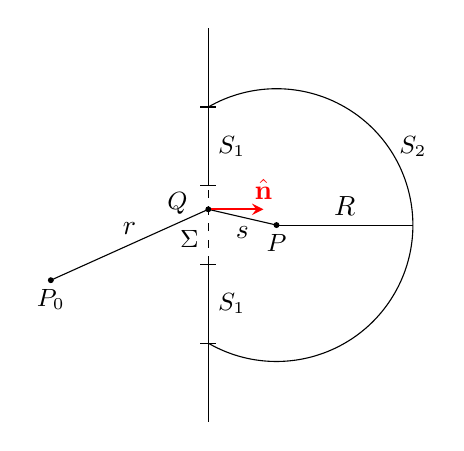
\begin{tikzpicture}

  \pgfmathsetmacro{\arcRadius}{1.5/sin(60)}
  \pgfmathsetmacro{\pX}{1.5/tan(60)}

  \draw[black] (0, .5) -- (0, 2.5);
  \draw[black] (0, -.5) -- (0, -2.5);
  \draw[dashed, black] (0, -.5) -- (0, .5);

  \foreach \y in {0.5, 1.5}{
      \draw[black] (-.1, \y) -- (.1, \y);
      \draw[black] (-.1, -\y) -- (.1, -\y);
    }

  \draw[black] (0, -1.5) arc (-120:120:\arcRadius);

  \coordinate (P0) at (-2, -0.7);
  \coordinate (P) at (\pX, 0);
  \coordinate (P1) at (\pX + \arcRadius,0);
  \coordinate (Q) at (0, 0.2);

  \draw[black] (P0) -- (Q) node[midway, above] {$r$};
  \draw[black] (Q) -- (P) node[midway, below] {$s$};
  \draw[black] (P) -- (P1) node[midway, above] {$R$};

  \draw[thick, red, -stealth] (Q) -- ++(.7,0) node[above] {$\hat{\mathbf{n}}$};

  \filldraw[black] (P0) circle (.03) node[below] {\small $P_0$};
  \filldraw[black] (Q) circle (.03)
  node[anchor=east, xshift=-4, yshift=2] {\small $Q$};
  \filldraw[black] (P) circle (.03) node[below] {\small $P$};

  \node[anchor=east, yshift=-5] at (0, 0) {\small $\Sigma$};
  \node[anchor=west] at (0, 1) {\small $S_1$};
  \node[anchor=west] at (0, -1) {\small $S_1$};
  \node[yshift=1cm] at (P1) {\small $S_2$};

\end{tikzpicture}
\end{document}